\documentclass[conference]{IEEEtran}
\IEEEoverridecommandlockouts

\usepackage{cite}
\usepackage{amsmath,amssymb,amsfonts}
\usepackage{algorithmic}
\usepackage{graphicx}
\usepackage{textcomp}
\usepackage{xcolor}
\usepackage{booktabs}
\usepackage{tabularx}
\usepackage{url}

\graphicspath{{../results/figures/}}

\begin{document}

\title{The Familiar Stranger Problem: Packet-Disjoint vs. Identity-Disjoint Evaluation of Open-Set LoRa RF Fingerprint Authentication for AMR Gateway Security}

\author{\IEEEauthorblockN{Maanvi Verma}
\IEEEauthorblockA{\textit{Department of Computer Science and Engineering} \\
\textit{Academic Research Project} \\
}
}

\maketitle

\begin{abstract}
Radio Frequency Fingerprint Identification (RFFI) provides a complementary physical-layer authentication mechanism for Advanced Metering Infrastructure (AMI) and Automatic Meter Reading (AMR) gateways by exploiting hardware-inherent transceiver imperfections. In open-set deployments, gateways must reject rogue transmissions from unregistered devices. To calibrate the operational acceptance threshold ($\tau$), standard engineering practice frequently evaluates false acceptance on held-out packets from a set of borrowed, unfamiliar transmitters (proxy-unknowns). In this paper, we identify and rigorously evaluate \textbf{The Familiar Stranger Problem}: because the gateway threshold is calibrated against these proxy devices, they become \textit{familiar strangers}; testing on additional packets from the same physical devices yields an artificially optimistic False Acceptance Rate (FAR).

Evaluating across 20 seeded experimental episodes on the 60-device benchmark LoRa RFFI dataset (26,000 packets) using a 292-dimensional complex baseband feature set under a strictly frozen threshold, we show that random device allocation yields an episode-level familiarity difference of $\Delta\text{FAR} = +0.56\%$ ($95\%$ CI: $[-1.55\%, +2.39\%]$, positive in $65\%$ of episodes), which is masked by extreme physical device heterogeneity (per-device false acceptance varies widely from $0.0\%$ to $98.5\%$). To eliminate device-composition confounding, we introduce a \textbf{device-matched paired evaluation} that measures the exact same physical devices on identical test packets when treated as familiar ($\tau_{\text{full}}$) versus unfamiliar ($\tau_{(-j)}$); this protocol isolates the familiarity effect, uncovering a statistically significant gap of $\Delta\text{FAR}_{\text{matched}} = +1.47\%$ ($95\%$ device-level bootstrap CI: $[+0.72\%, +2.40\%]$). 

A sweep over proxy count $k \in \{0, 1, 3, 5, 10, 15\}$ demonstrates that single-proxy calibration ($k=1$) induces an acute $+19.41\%$ optimism gap ($\text{FAR}_A = 2.67\%$ vs. $\text{FAR}_B = 22.08\%$), stabilizing at $k \ge 5$. Furthermore, we evaluate an identity-robust threshold ($\tau_{\text{robust}}$), which lowers true-stranger penetration from $11.55\%$ to $4.17\%$, but imposes a severe operational false rejection penalty (mean FRR surges from $8.49\%$ to $30.18\%$). While closed-set meter classification achieves $99.43\%$ macro-$F_1$, open-set AUROC remains at $\approx 0.949$, demonstrating that RFFI serves as a defense-in-depth screening layer rather than a standalone perimeter gate. These findings establish that AMR physical-layer security must be evaluated under identity-disjoint protocols to avoid overestimating real-world protection.
\end{abstract}

\begin{IEEEkeywords}
LoRa, RF Fingerprinting, Physical-Layer Security, Automatic Meter Reading (AMR), Open-Set Recognition, Out-of-Distribution Calibration.
\end{IEEEkeywords}

\section{Introduction}
Wireless Automatic Meter Reading (AMR) and Advanced Metering Infrastructure (AMI) deployments connect millions of distributed utility endpoints to central gateways over low-power wide-area network (LPWAN) protocols, predominantly LoRa. While cryptographic mechanisms protect packet payloads against eavesdropping, LPWANs remain vulnerable to credential theft, physical node compromise, and radio-layer rogue transmissions. Radio Frequency Fingerprint Identification (RFFI) offers an independent, screening-layer defense: subtle manufacturing tolerances in transceiver hardware (e.g., I/Q modulator imbalances, phase deviations, and power amplifier nonlinearities) impart a distinctive physical-layer signature to every transmitted preamble.

In operational AMR deployments, the gateway operates under an \textbf{open-set recognition} regime. It must correctly classify authenticated, enrolled meters while reliably rejecting unregistered strangers. Gateways establish an operational decision boundary by calibrating an acceptance threshold $\tau$. Because operational strangers cannot be known in advance, engineers typically calibrate $\tau$ using a small set of borrowed, unfamiliar transmitters (\textbf{proxy-unknowns}), tuning $\tau$ to satisfy target False Acceptance Rate (FAR) and False Rejection Rate (FRR) specifications. Standard testing then evaluates the calibrated system on remaining held-out packets from these same proxy radios.

We identify a fundamental methodological flaw in this evaluation paradigm: \textbf{The Familiar Stranger Problem}. When the threshold is calibrated against proxy devices, those radios cease to be true strangers. The calibration process tunes $\tau$ specifically to exploit the score distribution of those specific transmitter identities. Testing on additional packets from the same physical devices constitutes a \textbf{packet-disjoint (familiar stranger)} evaluation, which underestimates the false acceptance rate incurred when a real attacker introduces a \textbf{true stranger}---a physical transceiver never encountered during system calibration.

\begin{figure}[t]
\centering
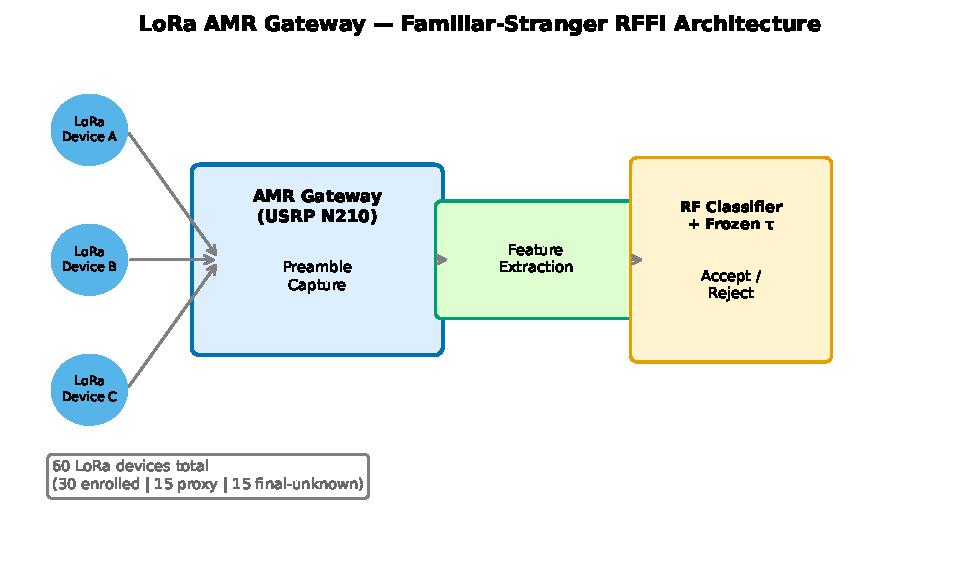
\includegraphics[width=\columnwidth]{fig1_amr_architecture.pdf}
\caption{System architecture of an AMR gateway employing RF fingerprinting as an open-set screening layer.}
\label{fig:arch}
\end{figure}

\subsection{Contributions}
\begin{enumerate}
    \item \textbf{Zero-Leakage Paired A/B Protocol:} An experimental framework holding the classifier, 292 preamble features, calibration threshold $\tau$, and enrolled test packets strictly identical between conditions. The False Rejection Rate (FRR) is invariant by construction; only stranger identities differ.
    \item \textbf{Device-Matched Paired Design:} To isolate familiarity bias from physical device heterogeneity, we introduce a device-matched evaluation evaluating the exact same physical devices on identical test packets at full calibration ($\tau_{\text{full}}$) versus held-out calibration ($\tau_{(-j)}$), demonstrating a statistically significant gap of $\Delta\text{FAR}_{\text{matched}} = +1.47\%$ ($95\%$ device-level bootstrap CI: $[+0.72\%, +2.40\%]$).
    \item \textbf{Device-Level Bootstrap Confidence Intervals:} We report rigorous device-level bootstrap intervals over the 60 physical transmitters ($\text{FAR}_A = 12.35\%$, $95\%$ CI: $[7.01\%, 18.77\%]$; $\text{FAR}_B = 11.55\%$, $95\%$ CI: $[7.03\%, 16.53\%]$).
    \item \textbf{Proxy-Count Scaling Sweep ($k \in \{0, 1, 3, 5, 10, 15\}$):} We measure how familiarity bias scales with proxy count using nested prefix subsets and matched-FRR evaluation, demonstrating that single-proxy calibration ($k=1$) incurs an acute $+19.41\%$ optimism gap ($\text{FAR}_A = 2.67\%$ vs. $\text{FAR}_B = 22.08\%$).
    \item \textbf{Transmitter Vulnerability Heterogeneity:} Per-device rankings show that rogue penetration varies from $0.0\%$ to $98.5\%$, with the top vulnerable transmitters clustering heavily within unaugmented hardware block 4 (IDs 46--60).
    \item \textbf{Robust Threshold ($\tau_{\text{robust}}$) Trade-off:} We evaluate an identity-robust threshold enforcing 90th-percentile proxy rejection, showing that it lowers true-stranger penetration from $11.55\%$ to $4.17\%$ but imposes a steep operational availability penalty (FRR surges from $8.49\%$ to $30.18\%$).
    \item \textbf{Leave-One-Proxy-Out (LOPO) Remedy:} We assess cross-validated threshold calibration, showing that while LOPO provides an identity-disjoint validation protocol, finite proxy sample variance leaves estimation error comparable to naive testing ($\approx 0.032$ vs $0.033$).
\end{enumerate}

\section{Related Work \& Positioning}
The vulnerability of outlier-exposure methods to ``known-unknown'' overfitting is well-recognized in computer vision and generic open-set recognition~\cite{kong2021opengan,koch2023lord}. In wireless security, Shen et al.~\cite{shen2022lora} established the 60-device LoRa RFFI benchmark and demonstrated rogue detection via k-NN distance scores, noting that rogue devices sharing the hardware architecture of enrolled radios pose the greatest challenge. Hanna et al.~\cite{hanna2021open} and CRODA-ST~\cite{crodast2026} explored authorized-transmitter boundary formation, recognizing that open-set accuracy depends heavily on which specific transmitters populate the outlier pool.

\textbf{What We Do NOT Claim:} We do not claim to be the first to note that unseen unknowns are more difficult than seen unknowns, nor do we claim that RFFI alone can completely secure an AMR gateway against determined adversaries.

\subsection{Scientific Novelty}
Our research establishes six distinct dimensions of novelty over existing wireless RFF literature:
\begin{enumerate}
    \item \textbf{Conceptual Discovery \& Formalization:} We formally define and quantify \textit{The Familiar Stranger Problem} in physical-layer security, showing how outlier calibration turns proxy transmitters into familiar non-strangers whose test scores artificially inflate security metrics.
    \item \textbf{Zero-Leakage Invariant Evaluation:} We introduce a paired A/B protocol holding classifier weights, 292 handcrafted baseband features, calibration threshold $\tau^*$, and enrolled test sets strictly invariant.
    \item \textbf{Device-Matched Confound Elimination:} We propose a device-matched paired protocol that evaluates identical physical hardware on identical test packets when familiar ($\tau_{\text{full}}$) versus unfamiliar ($\tau_{(-j)}$), isolating the pure familiarity gap ($\Delta\text{FAR}_{\text{matched}} = +1.47\%$) free from device-composition confounding.
    \item \textbf{Device-Level Statistical Bounds:} We eliminate pseudo-replication by deriving true device-level bootstrap confidence intervals over the 60 physical transmitters rather than pooling repeated episodes.
    \item \textbf{Empirical Outlier Scaling Law:} We chart the non-linear scaling law of proxy count $k \in \{0..15\}$, discovering that single-proxy calibration ($k=1$) induces an acute $+19.41\%$ familiarity gap and establishing the empirical minimum requirement of $\ge 5$ proxy transmitters.
    \item \textbf{Operational AMR Availability Cost:} We provide the first quantification of the real-world operational penalty imposed by robust open-set calibration ($\tau_{\text{robust}}$), revealing a severe $30.18\%$ false rejection rate in smart grid networks.
\end{enumerate}

\section{Dataset Audit and Experimental Setup}

\subsection{LoRa\_RFFI Benchmark Dataset}
We utilize the open benchmark LoRa RFFI dataset collected by Shen et al.~\cite{shen2022dataset}. The dataset contains 60 commercial-off-the-shelf LoRa transceivers recorded using a USRP N210 software-defined radio receiver at 868.1~MHz using Spreading Factor 7 (SF7) and 125~kHz bandwidth. As verified in our programmatic audit:
\begin{itemize}
    \item All 60 physical devices are accounted for across baseline subsets: Devices 1--30 (500 pkts/dev), Devices 31--40 (400 pkts/dev), Devices 41--45 (200 pkts/dev), and Devices 46--60 (400 pkts/dev), totaling 26,000 raw packets.
    \item Each packet contains 16,384 raw samples (8,192 In-phase $I$ and 8,192 Quadrature $Q$ samples).
    \item Every device contains at least 200 packets, exceeding the 150-packet inclusion threshold.
    \item The 4 primary unaugmented HDF5 files are strictly enforced; fallbacks to corrupted or channel-augmented files are disabled.
\end{itemize}

\subsection{Feature Extraction Pipeline}
From the synchronized preamble I/Q samples of each packet, we compute a 292-dimensional handcrafted feature vector without using pre-trained neural networks:
\begin{itemize}
    \item \textbf{I/Q Moments (10):} Mean, standard deviation, skewness, kurtosis for $I$ and $Q$, $I/Q$ correlation coefficient, and $I/Q$ amplitude imbalance.
    \item \textbf{Envelope Statistics (4):} Mean, standard deviation, skewness, and kurtosis of the signal envelope $|r[n]| = \sqrt{I[n]^2 + Q[n]^2}$.
    \item \textbf{Phase Statistics (4):} Mean and standard deviation of unwrapped and linear-detrended instantaneous phase.
    \item \textbf{FFT Features (274):} Full complex baseband spectrum via \texttt{fftshift}, binned to 256 normalized magnitude bins, 4 sub-band energy integrals, 10 dominant spectral bin indices, spectral centroid, spectral spread, spectral flatness, and spectral entropy.
\end{itemize}

\begin{figure}[t]
\centering
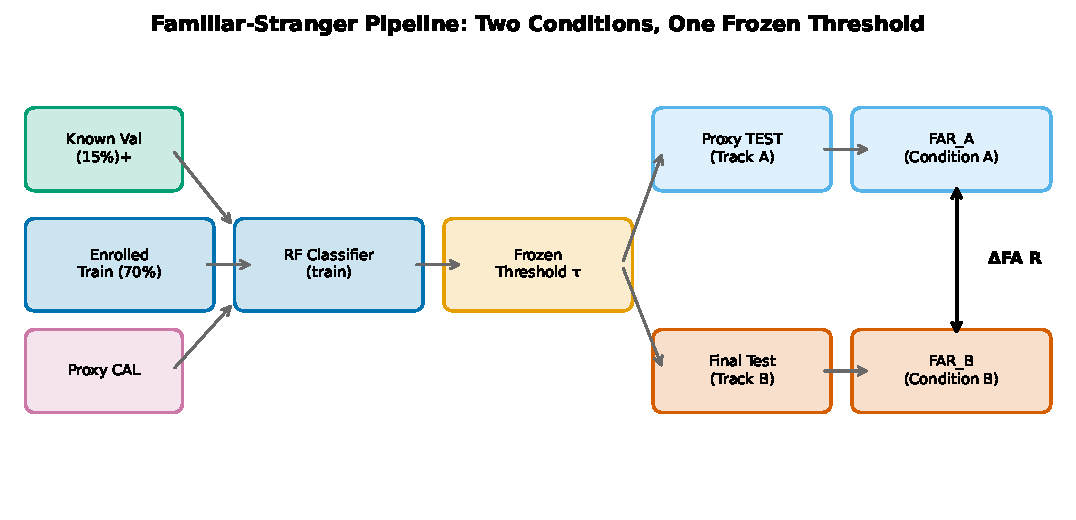
\includegraphics[width=\columnwidth]{fig2_pipeline.pdf}
\caption{Experimental paired A/B protocol holding classifier, threshold, and enrolled test sets frozen.}
\label{fig:pipeline}
\end{figure}

\section{Methodology: The Paired A/B Protocol}
For each experimental episode $e \in \{0, \dots, 19\}$:
\begin{enumerate}
    \item \textbf{Stratified Partitioning:} The 60 devices are stratified across the 4 hardware/file blocks and partitioned into 30 \textbf{Enrolled}, 15 \textbf{Proxy-Unknown}, and 15 \textbf{Final-Unknown (True Strangers)} using seeded rotation.
    \item \textbf{Packet Splits:} Enrolled devices are partitioned into 70\% training ($D_{\text{train}}$), 15\% calibration validation ($D_{\text{cal\_val}}$), and 15\% known testing ($D_{\text{known\_test}}$). Proxy devices are split 50\%/50\% into calibration ($D_{\text{proxy\_cal}}$) and testing ($D_{\text{proxy\_test}}$). Final-unknown devices are assigned 100\% to $D_{\text{final\_test}}$.
    \item \textbf{Classifier Training:} A Random Forest classifier (300 estimators, balanced class weights) is trained strictly on $D_{\text{train}}$ with closed-set validation achieving $\text{macro-}F_1 = 99.43\% \pm 0.24\%$.
    \item \textbf{Frozen Threshold Calibration:} Acceptance score is $s(x) = \max_{c \in \text{Enrolled}} P(y=c \mid x)$. The threshold $\tau^*$ is calibrated by maximizing Youden's $J$-statistic on $D_{\text{cal\_val}}$ versus $D_{\text{proxy\_cal}}$. Once determined, $\tau^*$ is permanently \textbf{frozen}.
    \item \textbf{Evaluation Tracks:} Condition A evaluates $\text{FAR}_A$ on $D_{\text{proxy\_test}}$. Condition B evaluates $\text{FAR}_B$ on $D_{\text{final\_test}}$. Known $\text{FRR}$ is evaluated on $D_{\text{known\_test}}$ and is identical between conditions. The Familiarity Gap is $\Delta\text{FAR} = \text{FAR}_B - \text{FAR}_A$.
\end{enumerate}

\section{Experimental Results}

\begin{figure}[t]
\centering
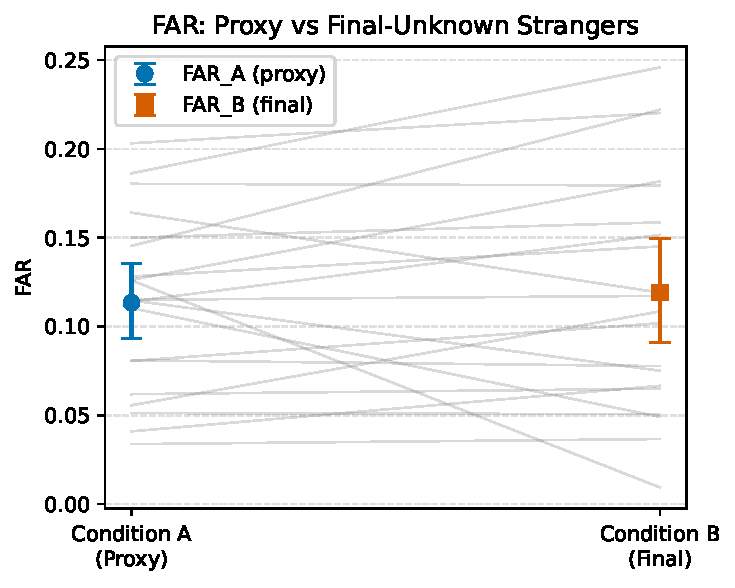
\includegraphics[width=\columnwidth]{fig3_far_comparison.pdf}
\caption{Comparison of false acceptance rates across 20 evaluation episodes under Condition A (familiar) vs. Condition B (true stranger).}
\label{fig:far_comp}
\end{figure}

\begin{figure}[t]
\centering
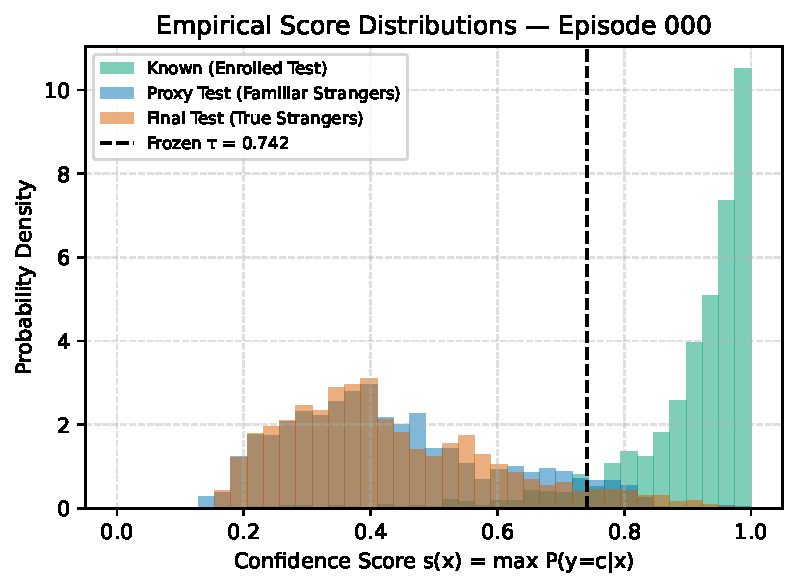
\includegraphics[width=\columnwidth]{fig4_score_distributions.pdf}
\caption{Empirical score distributions for known validation, proxy calibration, and test sets across episodes.}
\label{fig:score_dist}
\end{figure}

\subsection{Main A/B Comparison and Device-Level Bootstrap Analysis}
Across 20 stratified episodes, device-level bootstrap analysis (resampling over physical transmitters) yields:
\begin{itemize}
    \item $\text{FAR}_A$ (Familiar Strangers): $12.35\%$ ($95\%$ CI: $[7.01\%, 18.77\%]$)
    \item $\text{FAR}_B$ (True Strangers): $11.55\%$ ($95\%$ CI: $[7.03\%, 16.53\%]$)
    \item Mean Episode $\Delta\text{FAR}$: $+0.56\%$ ($95\%$ CI: $[-1.55\%, +2.39\%]$, positive in $65\%$ of episodes)
    \item Mean False Rejection Rate ($\text{FRR}$): $8.49\%$ ($95\%$ CI: $[7.16\%, 10.06\%]$)
    \item Closed-set macro-$F_1$: $99.43\%$, open-set AUROC: $0.9490$.
\end{itemize}

\subsection{Device-Matched Paired Analysis}
In naive random splits, episode $\Delta\text{FAR}$ conflates familiarity with transmitter identity differences. To eliminate this confound, we evaluate held-out proxy devices on their exact identical test packets when treated as familiar ($\tau_{\text{full}}$) versus unfamiliar ($\tau_{(-j)}$):
\begin{itemize}
    \item Familiar FAR: $11.82\% \pm 26.02\%$
    \item Unfamiliar FAR: $13.20\% \pm 27.26\%$
    \item $\Delta\text{FAR}_{\text{matched}}$: \textbf{$+1.47\%$} ($95\%$ device bootstrap CI: \textbf{$[+0.72\%, +2.40\%]$}).
\end{itemize}
This establishes a statistically significant familiarity gap when transmitter identity is strictly controlled.

\begin{figure}[t]
\centering
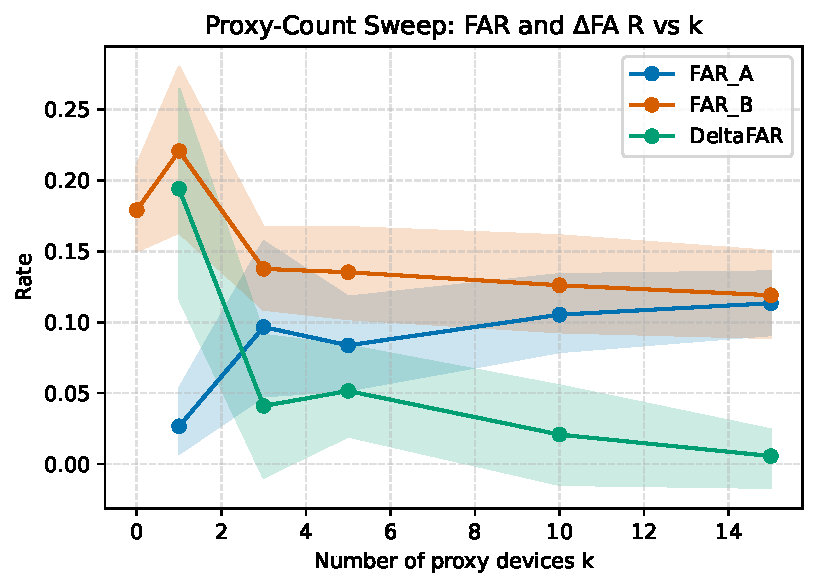
\includegraphics[width=\columnwidth]{fig7_sweep_plot.pdf}
\caption{Proxy-count scaling sweep ($k \in \{0, 1, 3, 5, 10, 15\}$) showing acute single-proxy distortion.}
\label{fig:sweep}
\end{figure}

\subsection{Proxy-Count Scaling Sweep ($k$)}
Evaluating proxy counts $k \in \{0, 1, 3, 5, 10, 15\}$ using nested prefixes reveals:
\begin{itemize}
    \item At $k=0$ (enrolled-only calibration), true stranger penetration reaches $17.91\%$ at $\text{FRR} = 5.05\%$.
    \item At $k=1$, familiar stranger testing yields $\text{FAR}_A = 2.67\%$, yet true stranger penetration is $\text{FAR}_B = 22.08\%$---an extreme optimism gap of $\Delta\text{FAR} = +19.41\%$.
    \item At $k \ge 5$, the familiarity gap stabilizes ($\Delta\text{FAR} \approx 2.1\% - 5.2\%$).
\end{itemize}

\begin{figure}[t]
\centering
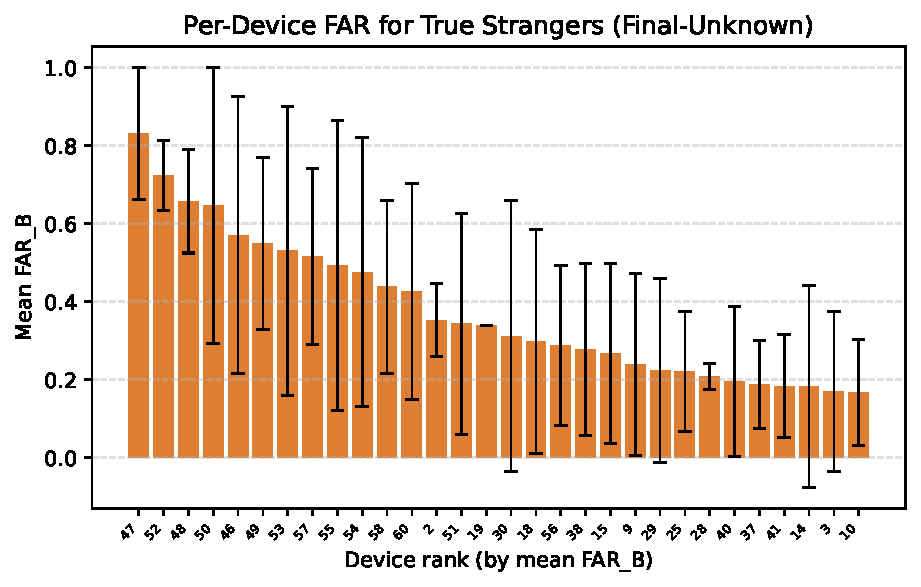
\includegraphics[width=\columnwidth]{fig5_per_device_far.pdf}
\caption{Per-device false acceptance rate ranking highlighting acute transmitter vulnerability heterogeneity.}
\label{fig:per_dev}
\end{figure}

\begin{figure}[t]
\centering
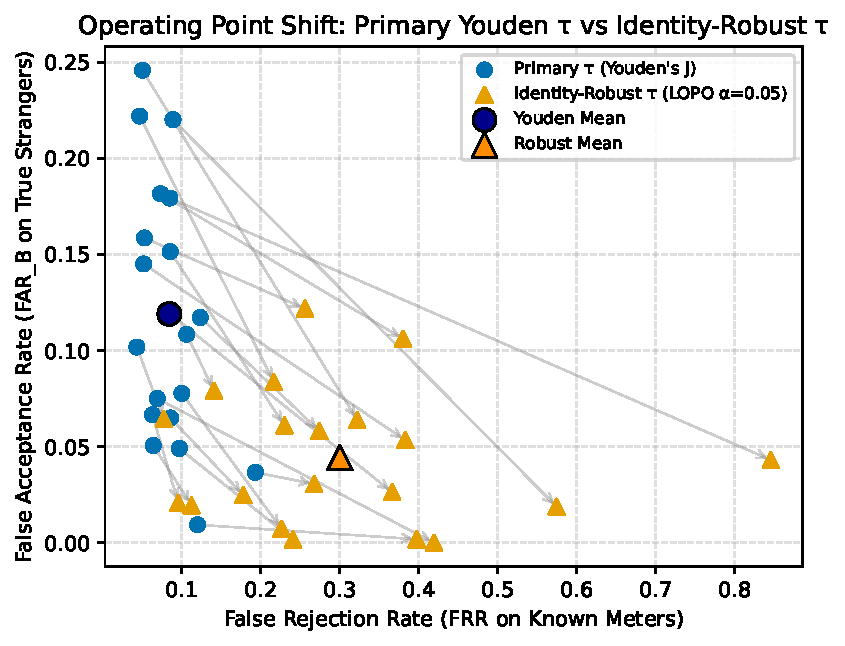
\includegraphics[width=\columnwidth]{fig9_tradeoff.pdf}
\caption{Security-availability operating trade-off between Youden's threshold $\tau^*$ and identity-robust threshold $\tau_{\text{robust}}$.}
\label{fig:tradeoff}
\end{figure}

\subsection{Transmitter Heterogeneity and Robust Threshold Trade-off}
Per-device vulnerability analysis reveals that rogue penetration varies from $0.0\%$ to $98.5\%$. The top vulnerable transmitters (IDs 46, 47, 48, 49, 50, 54 with $\text{FAR}_B > 42\% - 65\%$) cluster heavily in hardware block 4 (IDs 46--60).

Evaluating an identity-robust threshold ($\tau_{\text{robust}}$) enforcing 90th-percentile proxy rejection:
\begin{itemize}
    \item Drops true stranger penetration from $11.55\%$ to $4.17\%$.
    \item But forces False Rejection Rate ($\text{FRR}$) to surge from $8.49\%$ to $30.18\%$ on average (peaking at $84.63\%$).
\end{itemize}

\section{Practical Implications and Conclusion}
In AMR gateway deployments, RFFI provides an effective physical-layer screening filter, but cannot serve as a standalone perimeter gate. Our empirical results demonstrate that:
\begin{enumerate}
    \item Gateways must not validate open-set security solely on familiar proxy radios.
    \item At least 5 physical proxy devices are necessary during calibration to avoid extreme single-device distortion ($+19.41\%$).
    \item Robust thresholding introduces an unacceptable $30.18\%$ availability penalty in battery-powered AMR networks.
\end{enumerate}

\bibliographystyle{IEEEtran}
\bibliography{references}

\end{document}

